% Chapter Template

\chapter{Experiment} % Main chapter title

\label{Chapter4} % Change X to a consecutive number; for referencing this chapter elsewhere, use \ref{ChapterX}

As exposed more thoroughly in Section \ref{sec:issues}, we have encountered some issues that forced us to reschedule the experiment described here, and we will be performing it after writing this report. The present chapter however exposes the experiment as we intend to run it.

The goal of this experiment is to try to estimate the limits of self attribution of a distorted movement. We will do so by estimating the just noticeable difference (JND) in visual stimuli discrepancy. This means estimating the just noticeable \textit{distortion} made to the movement and hence the visual stimuli. The JND is estimated by using the adaptive staircase method introduced by Meese \cite{meese1995using}.

This method tries to estimate the JND by finding the point at which the subjects are uncertain whether a given visual stimuli corresponds to the actual movement they performed. These are found by changing the intensity of the distortion, based on whether the subject judged the last trial as distorted or not, and the JND is computed as the mean of the last few staircase turns (i.e.\ going from an increasing trend to a decreasing one or vice-versa). The detection judgment is gathered using a Yes/No prompt called the detection question : ``Did the movements you saw exactly correspond to the movements you performed?''

\section{Just Noticeable Difference}

The JND will be measured in term of $\gamma$, the gain of the distortion function introduced in Equation \ref{eq:DistortionFunction}. In general, if $\gamma = \SI{-3}{\decibel}$ the subjects are hindered by having to travel two times the distance between the targets, whereas if $\gamma = \SI{3}{\decibel}$ the movement will be amplified and the required motion will be reduced by $50\%$.

Due to the nature of the Egocentric Coordinates and how the distortion is applied (respectively detailed in Chapters \ref{Chapter2} and \ref{Chapter3}), this will not exactly be a metric of the difference in the distance that the subjects have to cover in order to reach the target, such as the metric used by \cite{debarba2017embodiment}. It however gives a good understanding of the strength and the effect of the applied distortion.

\section{Equipment and Software}

The HMD used for this experiment is going to be the Oculus Rift in its first consumer version, with a resolution of $1080 \times 1200$ pixels per eye and a refresh rate of \SI{90}{\hertz}. Head orientation is acquired using the internal sensors of the HMD in order to minimize latency, and its orientation drift around the vertical axis is corrected using a set of markers placed on it. These markers also serve to determine the position of the camera in the virtual environment.

Audio is delivered using a pair of Bose\textsuperscript{\textregistered} QuietComfort 35 wireless headphones. They feature high quality environmental noise cancellation and are additionally used to stream unlocalized white noise, in order to fully isolate the subjects. If needed, they are also used as a communication means between the subject and experimenter, the latter making use of a microphone.

Motion capture is performed using a PhaseSpace Impulse X2 optical tracking system. The setup uses 18 infrared cameras and a suit equipped with 38 LED markers, which are arranged as described by Molla \cite{molla2016precise} in order to track limb rigid bodies.

The virtual environment was developed using the Unity game engine. The room setup is derived from \cite{debarba2017embodiment} with a chair, a carpet, and a few point light sources. The carpet is here to better match the real world, in which the tracking space has a carpet on its floor. The physical chair has been measured so that it would match the virtual seat we are using. Additionally, the wall in front of the subject features textual information on the next target to be hit, or on resting times.

The avatar is animated using the IK and retargeting algorithms proposed by Molla et al.\ \cite{molla2013singularity,molla2017egocentric}, the latter of which is modified as described in Chapter \ref{Chapter3}.

\section{Experiment design}

We will manipulate three factors: the sign of the distortion (positive or negative), respectively yielding a helped and hindered movement, the starting value of that distortion (\num{0} or \SI{3}{\decibel}, and the target sequence (see below). Chapter \ref{Chapter3} gives a complete overview of the concept of distortion and its sign, as well as how it is implemented.

\subsection{Task}
\label{sec:task}

\begin{wrapfigure}{i}{.4\textwidth}
    \center{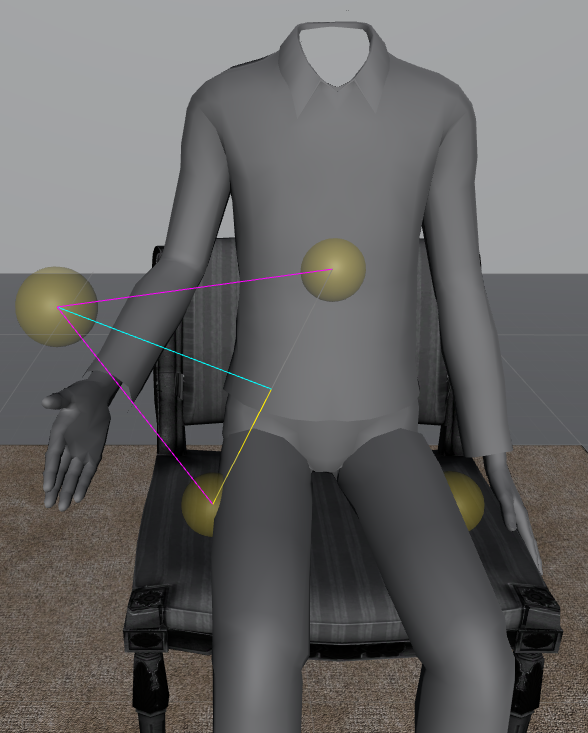
\includegraphics[width=.39\textwidth]
    {Figures/target_placement.png}}
    \caption{An example of target placement with lines showing how its position was reconstructed. The magenta lines are the one of desired length.}\label{fig:targetPlacement}
\end{wrapfigure}

While the whole set of IK goals will be distorted during the experiment, we will be focusing on the dominant hand movement. The task is performed in a seated position in order to avoid any unnecessary movement of the lower limbs, and has the subjects reach three targets. One of them may be in the air in front of them, while the starting and finishing location is the same relative to their skin. The reaching task is performed with the directing hand, and the subjects are instructed to keep their other hand at their side.

There are four different target orders: \textbf{Chest-Air-Chest} ($O_1$), \textbf{Leg-Air-Leg} ($O_2$), \textbf{Chest-Leg-Chest} ($O_3$), and \textbf{Leg-Chest-Leg} ($O_4$). The targets are located as depicted on Figure \ref{fig:targetPlacement} and the leg target is picked according to the subject's handedness: left-handed subjects for instance will have to reach for their left thigh. The first target to be displayed, $T_1$, is always one on the skin and requires the subjects to perform a self-contact in order to activate it. After a random time between \num{200} and \SI{300}{\milli\second}, the target activates. Then the subject moves the hand to the next target, which activates after \SI{100}{\milli\second}. Once this is done the subject goes back to $T_1$, and the detection question is finally asked.

If the sequence requires an intermediary air target ($O_1$ and $O_2$), that target's position is computed such that the subjects have to move a predefined distance $d = 75\%$ of arm length between $T_1$ and $T_{\text{air}}$. Given that a whole sphere of positions is possible, and in order to disambiguate that position, we require that $T_\text{air}$ is also at the same distance $d$ from the third, unused target $T_3$. The air target position therefore is on the intersection between the two spheres of radius $d$ centered on $T_1$ and $T_3$, and we chose the topmost position as a reasonable last disambiguation criterion. Figure \ref{fig:targetPlacement} shows how such position is computed. This target placement is useful in that it helps requiring movements of equal effort and does not change the ability to perform the trials across subjects.

One trial---or staircase run---consists of a reaching task, followed by the detection question. Based on the answer to this question, the experiment software modifies the distortion for the next staircase run as follows:
\begin{quote}
    \begin{labeling}{"No" and $\gamma = 0$}
      \item ["Yes"] The discrepancy is increased.
      \item ["No" and $\gamma \neq 0$] The discrepancy is decreased.
      \item ["No" and $\gamma = 0$] The parameter is not changed\footnote{We do not change the distortion in this case because this would invert the sign of the distortion, thus introducing a distortion of different sign.}.
    \end{labeling}
\end{quote}

The amount of each increment or decrement is dynamic: it starts at \num{0.5} and is halved after the first staircase turn. That value is then kept for the rest of that staircase. This helps going quickly from the starting distortion to the point where subjects are unsure whether the movement they saw was theirs, and then explores the space around that point.

\begin{figure}[h]
    \center{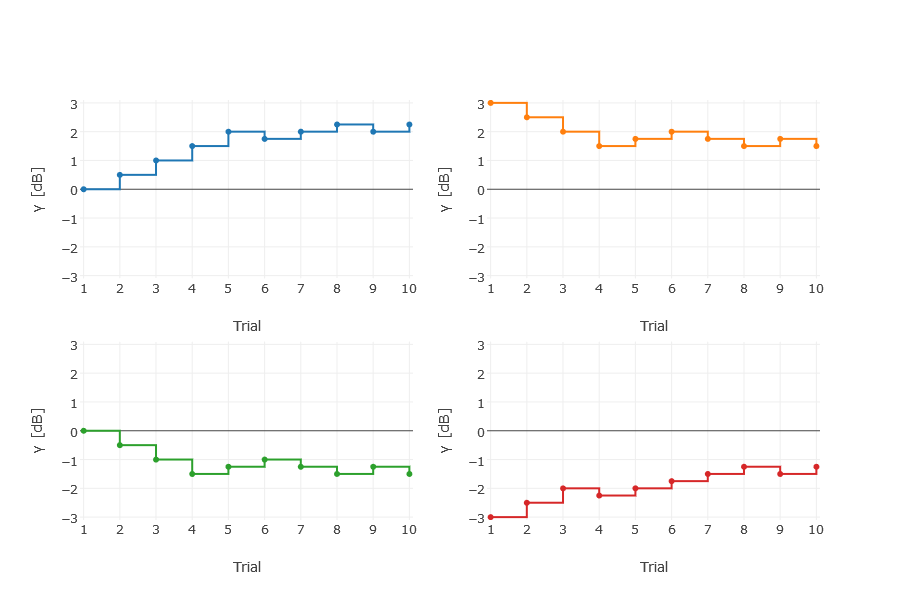
\includegraphics[width=\textwidth]
    {Figures/trials.png}}
    \caption{Four made up partial instances of staircases. Each one features ten trials and four staircases turns, including the one happening in the last trial. The sign of the staircase is the same for each row, while the starting distortion is the same for each column.}\label{fig:trials}
\end{figure}

A staircase is completed either when the subjects change direction 7 times or when they performed 20 trials in that staircase. Figure \ref{fig:trials} shows four instances of ten consecutive trial, depicting the four different initial staircases configuration used for each possible target order.

\section{Hypotheses}

Considering the target orders we introduced in Section \ref{sec:task}, namely \textbf{Chest-Air-Chest} ($O_1$), \textbf{Leg-Air-Leg} ($O_2$), \textbf{Chest-Leg-Chest} ($O_3$), and \textbf{Leg-Chest-Leg} ($O_4$), and their resulting JNDs, denoted $\text{JND}_n$, the hypotheses we have for the experiment are the following:

\begin{quote}
    \begin{labeling}[:]{H2}
      \item [H1] The absolute value of all JNDs will be higher when the distortion is positive.
      \item [H2] For a positive distortion, $\text{JND}_3 \approx \text{JND}_4$
      \item [H3] Also for a positive distortion, $\text{JND}_1 < \text{JND}_2 < \text{JND}_3$
      \item [H4] For a negative distortion, $\text{JND}_1 > \text{JND}_2$
    \end{labeling}
\end{quote}

H1 is based on the findings of \cite{debarba2017embodiment}, who found that a hindering movement distortion is more quickly detected than a helping one. The justifications for all other hypotheses are based on the type of movement asked of the subjects.

Considering the similarity of the tasks $O_3$ and $O_4$, we believe they will exhibit similar JNDs, hence H2.

H3 translates our belief that the presence or not of body parts other than the starting one (the leg in the case of $O_2$ for instance) along the path of movement have an impact on the detection threshold. The symmetry of the repartition of the said body parts when performing $O_1$ (i.e.\ the legs below and the head above) will be beneficial to the resulting motion, whereas having the whole chest on one side of the task $O_2$ and nothing on the other one will lead to an increased JND. Similarly, both $O_3$ and $O_4$ will be negatively affected due to the nature of their respective paths. Differences in acceptable thresholds depending on the direction of movement have also been observed in the case of a more uniformly distorted space, as reported by Burns et al.\ \cite{burns2007macbeth}, but this is of lesser interest to us because we believe the influence of other body parts will be greater.

Also reasoning about trajectories, we believe that a negative distortion will have a more visible impact on $O_1$ than on $O_2$, as stated by H4. The reason for this is that on a vertical path starting on the leg, subjects may travel a longer distance before reaching the joint limits of their arm, as opposed to during a horizontal trajectory starting at the chest. Indeed, the further one can go from the chest is roughly one arm's length, whereas starting from the leg allows one to reach higher.

\section{Procedure}

The procedure of the experiment is planned to be the one described in the following lines.

The subjects are welcomed and introduced to the protocol described here, and then introduced to the tracking equipment. A consent form is signed and a characterization form is then filled in by the subjects. The questionnaire features background questions such as age and handedness, but also regarding any previous VR experiment participation, or experience with HMDs. They are then asked to remove their shoes and helped putting the motion capture suit on. A calibration is then performed as described by \cite{molla2017egocentric}.

Before beginning the actual staircase trials, a familiarization phase takes place. The subjects go through two series of five trials with constant distortion. The first one has no distortion at all and the second has a big one of $\gamma = \SI{3}{\decibel}$. The subjects are instructed to always answer ``Yes'' during the first staircase, and ``No'' during the second one, so that they become familiar with the whole procedure.

After these training trials, the real staircases begin. In order to prevent the sequential presentation of trials in the same staircase, four staircases are executed in parallel as long as the number of trials left permits it. As described earlier, each staircase ends either after 20 trials, or when seven staircase turns are registered. At the end of each staircase there is a time for the subject to rest, during which they are encouraged to ask for a glass of water if they so desire. If they do, the experimenter helps them with the handling of the headphones and HMD. When they are ready to continue, the experimenter presses a button in order to resume the experiment with the next series of trials.

\section{Subjects}

A few physical limitations will be applied to filter the subjects of this experiment. Their height will be required to be between smaller than 180cm and have a body mass index between 18 and 27. Those criteria are due to our motion capture equipment and especially the size of the suit on which the markers are placed. We also require that they have a normal or corrected to normal vision, and be fluent in both written and spoken English.

The subjects will be paid CHF 20.- per hour for their participation in the experiment.
